%%%%%%%%%%%%%%%%%%%%%%%%%%%%%%%%%%%%%%%%%%%%%%%%%%%%%%%%%%%%%%%%%%%%%%
% Lớp 12 | Nguyên hàm, tích phân | Tích phân
% Dạng 2D4?2-1: Công thức lý thuyết
% Số câu: 51  (sinh tự động bởi tach_cau.py; từ nay thầy sửa trực tiếp file này)
%%%%%%%%%%%%%%%%%%%%%%%%%%%%%%%%%%%%%%%%%%%%%%%%%%%%%%%%%%%%%%%%%%%%%%

%%%%%%%%%%%%%%%% TRẮC NGHIỆM 4 PHƯƠNG ÁN %%%%%%%%%%%%%%%%

% nguồn: Phan1_Lop_12_Dai_so_Chuong_4
\begin{ex}%[2D4N2-1]%[ma:72de2cc1]
	 Cho $f(x)$ là hàm số liên tục trên đoạn $[a;b]$ và $c \in[a;b]$. Tìm mệnh đề đúng trong các mệnh đề sau.
	 \choice
		{$\displaystyle\int_{a}^{c} f(x)\mathrm{\,d}x+\displaystyle\int_{c}^{b}  f(x) \mathrm{\,d}x=\displaystyle\int_{b}^{a} f(x) \mathrm{\,d}x$}
		{$\displaystyle\int_{a}^{b} f(x)\mathrm{\,d}x+\displaystyle\int_{a}^{c} f(x)  \mathrm{\,d}x=\displaystyle\int_{c}^{b} f(x)\mathrm{\,d}x$}
		{$\displaystyle\int_{a}^{b} f(x)\mathrm{\,d}x-\displaystyle\int_{a}^{c}  f(x) \mathrm{\,d}x=\displaystyle\int_{b}^{c} f(x)\mathrm{\,d}x$}
		{\True $\displaystyle\int_{a}^{b} f(x)\mathrm{\,d}x+\displaystyle\int_{c}^{a}  f(x) \mathrm{\,d}x=\displaystyle\int_{c}^{b} f(x)\mathrm{\,d}x$}
	\loigiai{ 
		Theo tính chất của tích phân ta có $\displaystyle\int_{a}^{b} f(x) \mathrm{\,d}x+\displaystyle\int_{c}^{a} f(x) \mathrm{\,d}x=\displaystyle\int_{c}^{b} f(x) \mathrm{\,d}x$. 
	 }
\end{ex}

% nguồn: Phan1_Lop_12_Dai_so_Chuong_4
\begin{ex}%[2D4N2-1]%[ma:62e42dae]
	Cho hàm số $f(x)$ liên tục trên  đoạn $[a;b]$ và số thực $k\in[a;b]$. Phát biểu nào sau đây đúng?
	 \choice
		 {\True $\displaystyle\int_{a}^{b}f(x)\mathrm{\,d}x=\displaystyle\int_{a}^{k}f(x)\mathrm{\,d}x+\displaystyle\int_{k}^{b}f(x)\mathrm{\,d}x$}
		 {$\displaystyle\int_{a}^{b}f(x)\mathrm{\,d}x=\displaystyle\int_{k}^{a}f(x)\mathrm{\,d}x+\displaystyle\int_{k}^{b}f(x)\mathrm{\,d}x$}
		 {$\displaystyle\int_{a}^{b}f(x)\mathrm{\,d}x=\displaystyle\int_{a}^{k}f(x)\mathrm{\,d}x+\displaystyle\int_{b}^{k}f(x)\mathrm{\,d}x$}
		{$\displaystyle\int_{a}^{b}f(x)\mathrm{\,d}x=\displaystyle\int_{b}^{k}f(x)\mathrm{\,d}x+\displaystyle\int_{k}^{a}f(x)\mathrm{\,d}x$} 
	 \loigiai{
		Phát biểu  đúng là $\displaystyle\int_{a}^{b}f(x)\mathrm{\,d}x=\displaystyle\int_{a}^{k}f(x)\mathrm{\,d}x+\displaystyle\int_{k}^{b}f(x)\mathrm{\,d}x$.
	} 
\end{ex}

% nguồn: Phan1_Lop_12_Dai_so_Chuong_4
\begin{ex}%[2D4N2-1]%[ma:762ef3de]
	Cho hàm số $f(x)$ có đạo hàm $f'(x)$ liên tục  trên $\mathbb{R}$ và $f(2)=3$, $f(5)=2$. Giá trị của $\displaystyle\int_2^5{f'(x)} \mathrm{\,d}x$ bằng
	\choice 
		{\True  $-1$}
		 {$1$}
		 {$5$}
		 {$6$}
	\loigiai{ 
		 $$\displaystyle\int_2^5{f'(x)} \mathrm{\,d}x = \left. f(x)\right|_2^5 = f(5)-f(2)=2-3=-1.$$
	 }
\end{ex}

% nguồn: Phan1_Lop_12_Dai_so_Chuong_4
\begin{ex}%[2D4N2-1]%[ma:aa5ef5e0]
	Cho $\displaystyle\int_0^1f(x)\mathrm{\,d}x=-1$; $\displaystyle\int_0^3f(x)\mathrm{\,d}x=5$. Giá trị của $\displaystyle\int_1^3f(x)\mathrm{\,d}x$ bằng 
	\choice 
		{$4$} 
		{$1$} 
		 {$5$}
		{\True $6$} 
	\loigiai{ 
		Ta có  $\displaystyle\int_1^3f(x)\mathrm{\,d}x=\displaystyle\int_0^3f(x)\mathrm{\,d}x-\displaystyle\int_0^1f(x)\mathrm{\,d}x=5-(-1)=6$.
	} 
\end{ex}

% nguồn: Phan1_Lop_12_Dai_so_Chuong_4
\begin{ex}%[2D4N2-1]%[ma:267c8a4f]
	Cho hàm số $y=f(x)$ liên tục trên $\mathrm{R}$, $\displaystyle\int_3^5 f(x)\mathrm{\,d}x =2$. Biểu thức  $\displaystyle\int_5^3 f(x)\mathrm{\,d}x$ bằng
	\choice 
		{$2$} 
		 {$\dfrac{1}{2}$}
		 {\True $-2$}
		{$-\dfrac{1}{2}$} 
	 \loigiai{
		 $\displaystyle\int_5^3 f(x)\mathrm{\,d}x = - \displaystyle\int_3^5 f(x)\mathrm{\,d}x = -2$.
	} 
\end{ex}

% nguồn: Phan1_Lop_12_Dai_so_Chuong_4
\begin{ex}%[2D4N2-1]%[ma:de15c72c]
	 Nếu $\displaystyle\int_2^5f(x)\mathrm{\,d}x=2$ thì $\displaystyle\int_5^2f(x)\mathrm{\,d}x$ bằng
	 \choice
		{\True  $-2$}
		{$2$} 
		{$-5$} 
		{$5$} 
	 \loigiai{
		 Ta có $\displaystyle\int_5^2f(x)\mathrm{\,d}x=-\displaystyle\int_2^5f(x)\mathrm{\,d}x=-2$.
	} 
\end{ex}

% nguồn: Phan1_Lop_12_Dai_so_Chuong_4
\begin{ex}%[2D4N2-1]%[ma:de58e752]
	Cho $F(x)$ là một nguyên hàm của hàm số $y=f(x)$ trên  đoạn $[a; b]$. Tìm khẳng định đúng
	 \choice
		{\True $\displaystyle\int_a^b f(x)\mathrm{\,d}x=F(b)-F(a)$} 
		 {$\displaystyle\int_a^b f(x)\mathrm{\,d}x=f(b)-f(a)$}
		 {$\displaystyle\int_a^b f(x)\mathrm{\,d}x=f(b)+f(a)$}
		 {$\displaystyle\int_a^b f(x)\mathrm{\,d}x=F(b)+F(a)$}
	 \loigiai{
		 Cho $F(x)$ là một nguyên hàm của hàm số $y=f(x)$ trên đoạn $[a; b]$, khi đó
		\[ 
		\displaystyle\int_a^b f(x)\mathrm{\,d}x=F(b)-F(a). 
		 \]
	 }
\end{ex}

% nguồn: Phan1_Lop_12_Dai_so_Chuong_4
\begin{ex}%[2D4N2-1]%[ma:6bec2d79]
	Khẳng định nào trong các khẳng định sau đúng với mọi hàm $f(x)$, $g(x)$ liên tục trên $K$ và $a$, $b$ là các số bất kỳ  thuộc $K$?
	\choice 
		{\True $\displaystyle\int_a^b\left[f(x)+2\right]\mathrm{\,d}x=\displaystyle\int_a^b  f(x)\mathrm{\,d}x+2\displaystyle\int_a^b \mathrm{\,d}x$}
		{$\displaystyle\int_a^b \dfrac{f(x)}{g(x)}\mathrm{\,d}x=\dfrac{\displaystyle\int_a^b f(x)\mathrm{\,d}x}{\displaystyle\int_a^b g(x)  \mathrm{\,d}x}$}
		{$\displaystyle\int_a^b\left[f(x) \cdot g(x)\right] \mathrm{\,d}x=\displaystyle\int_a^b f(x) \mathrm{\,d}x \cdot \displaystyle\int_a^b g(x) \mathrm{\,d}x$} 
		{$\displaystyle\int_a^b f^2(x) \mathrm{\,d}x=\left[\displaystyle\int_a^b  f(x) \mathrm{\,d}x\right]^2$}
	 \loigiai{
		Theo tính chất  tích phân ta có
	$\displaystyle\int_a^b\left[f(x)+2\right] \mathrm{\,d}x=\displaystyle\int_a^b f(x) \mathrm{\,d}x+\displaystyle\int_a^b 2  \mathrm{\,d}x=\displaystyle\int_a^b f(x)\mathrm{\,d}x+2\displaystyle\int_a^b \mathrm{\,d}x$ .}
\end{ex}

% nguồn: Phan1_Lop_12_Dai_so_Chuong_4
\begin{ex}%[2D4N2-1]%[ma:4d12eb7f]
	Cho hàm số $f(x)$ có một nguyên hàm trên $\mathbb{R}$  là $F(x)$. Biết $F(1)=3$ và $F(3)=-2$, giá trị của $I=\displaystyle\int_{1}^{3}f(x)\mathrm{\,d}{x}$ bằng
	 \choice
		 {$I=5$}
		 {$I=1$}
		{$I=-1$} 
		{\True  $I=-5$}
	\loigiai{ 
		 $I=\displaystyle\int_{1}^{3}f(x)\mathrm{\,d}{x}=\left.F(x)\right|_{1}^{3}=F(3)-F(1)=-2-3=-5$.
	} 
\end{ex}

% nguồn: Phan1_Lop_12_Dai_so_Chuong_4
\begin{ex}%[2D4N2-1]%[ma:78cdc523]
	Cho hàm số $f(x)$ liên tục trên $\mathbb{R}$ và $\displaystyle\int_0^3 f(x)\,\mathrm{\,d}x = 3$. Giá trị của tích phân $\displaystyle\int_0^3 2f(x)\,\mathrm{\,d}x$  là
	\choice 
		 {$1$}
		 {$4$}
		{\True  $6$}
		 {$5$}
	 \loigiai{
		Ta  có
	\[\displaystyle\int_0^3 2f(x)\,\mathrm{\,d}x=2\int_0^3 f(x)\,\mathrm{\,d}x=2 \cdot 3 =6.\]} 
\end{ex}

% nguồn: Phan1_Lop_12_Dai_so_Chuong_4
\begin{ex}%[2D4N2-1]%[ma:be437479]
	Cho hàm số $f(x)$ liên tục trên $\mathbb{R}$ thỏa mãn $\displaystyle\int_{0}^{-1} f(x) \mathrm{\,d}x=6$,  $\displaystyle\int_{0}^{1} f(x) \mathrm{\,d}x=8$. Khi đó giá trị $\displaystyle\int_{-1}^{1} \frac{f(x)}{2} \mathrm{\,d}x$ bằng
	\choice 
		 {$14$}
		{\True $1$} 
		 {$4$}
		{$2$} 
	\loigiai{ 
		Ta có $\displaystyle\int_{-1}^{1} \dfrac{f(x)}{2} \mathrm{\,d}x=\dfrac{1}{2}\displaystyle\int_{-1}^{0} f(x) \mathrm{\,d}x+\dfrac{1}{2}\displaystyle\int_{0}^{1}  f(x) \mathrm{\,d}x =\dfrac{1}{2}(-6+8)=1$.
	 }
\end{ex}

% nguồn: Phan1_Lop_12_Dai_so_Chuong_4
\begin{ex}%[2D4N2-1]%[ma:6a61cb3f]
	Cho hàm số $y=F(x)$  là một nguyên hàm của hàm số $f(x)$ trên tập $\mathscr{K}$ và $a,b\in \mathscr{K}$. Khẳng định nào sau đây \textbf{đúng}?
	 \choice
		{\True  $ \displaystyle\int_{a}^{b}f(x)\mathrm{\,d}x=F(b)-F(a)$}
		{$ \displaystyle\int_{a}^{b}f(x)\mathrm{\,d}x=F(a)-F(b)$} 
		{$  \displaystyle\int_{a}^{b}f(x)\mathrm{\,d}x=F(b)+F(a)$}
		 {$ \displaystyle\int_{a}^{b}f(x)\mathrm{\,d}x=F(b)\cdot F(a)$}
	\loigiai{ 
		Ta có $ \displaystyle\int_{a}^{b}f(x)\mathrm{\,d}x=F(b)-F(a)$. 
	} 
\end{ex}

% nguồn: Phan1_Lop_12_Dai_so_Chuong_4
\begin{ex}%[2D4N2-1]%[ma:5f38faa1]
	 Cho $\displaystyle\int_1^2f(x)\mathrm{\,d}x=10$. Tính $\displaystyle\int_2^1f(x)\mathrm{\,d}x$.
	\choice 
		{\True  $-10$}
		 {$10$}
		 {$5$}
		{$-5$} 
	 \loigiai{
	 Ta có $\displaystyle\int_2^1f(x)\mathrm{\,d}x=-\displaystyle\int_1^2f(x)\mathrm{\,d}x=10$. }
\end{ex}

% nguồn: Phan1_Lop_12_Dai_so_Chuong_4
\begin{ex}%[2D4N2-1]%[ma:e6c25cbd]
	Cho hàm số $y=f(x)$  liên tục trên $\mathrm{R}$, $\displaystyle\int_6^7 f(x)\mathrm{\,d}x =4$. Biểu thức $\displaystyle\int_6^7 20f(x)\mathrm{\,d}x$ bằng
	\choice 
		{\True  $80$}
		{$24$} 
		 {$16$}
		 {$5$}
	 \loigiai{
		$\displaystyle\int_6^7 20f(x)\mathrm{\,d}x  = 20\displaystyle\int_6^7 f(x)\mathrm{\,d}x = 20 \cdot 4 = 80$.
	} 
\end{ex}

% nguồn: Phan1_Lop_12_Dai_so_Chuong_4
\begin{ex}%[2D4N2-1]%[ma:4470410f]
	Cho hàm  số $y = f(x)$ liên tục trên đoạn $[a;b]$. Gọi $F(x)$ là một nguyên hàm của hàm số $f(x)$ trên đoạn $[a;b]$. Khẳng định nào sau đây \textbf{sai}?
	 \choice
		{$\displaystyle\int_a^b f(x) \mathrm{\,d}x = \int_a^c f(x) \mathrm{\,d}x + \int_c^b f(x) \mathrm{\,d}x \quad (a < c < b)$} 
		{$\displaystyle\int_a^b \left[f(x) - g(x) \right] \mathrm{\,d}x = \int_a^b f(x) \mathrm{\,d}x - \int_a^b g(x)  \mathrm{\,d}x$}
		 {\True $\displaystyle\int_a^b f(x) \mathrm{\,d}x = F(a) - F(b)$}
		{$\displaystyle\int_a^b f(x) \mathrm{\,d}x =  -\int_b^a f(x) \mathrm{\,d}x$}
	 \loigiai{
		Ta  có $\displaystyle\int_a^b f(x) \mathrm{\,d}x = F(b) - F(a)$.
	 }
\end{ex}

% nguồn: Phan1_Lop_12_Dai_so_Chuong_4
\begin{ex}%[2D4N2-1]%[ma:45bbc181]
	\immini{Diện tích của hình phẳng phần gạch chéo trong hình bên được tính theo công thức nào  sau đây?
	\choice 
		{\True  $S=\displaystyle\int^2_0f(x)\mathrm{\,d}x-\displaystyle\int^4_2f(x)\mathrm{\,d}x$}
		 {$S=-\displaystyle\int^2_0f(x)\mathrm{\,d}x+\displaystyle\int^4_2f(x)\mathrm{\,d}x$}
		 {$S=\displaystyle\int^2_0f(x)\mathrm{\,d}x+\displaystyle\int^4_2f(x)\mathrm{\,d}x$}
		 {$S=\displaystyle\int^4_0f(x)\mathrm{\,d}x$}}
		{\begin{tikzpicture}[scale=1,font=\footnotesize,line join=round,line cap=round,>=stealth]
		 \tikzset{every node/.style={scale=0.9}}
		\draw[->] (-1.1,0)--(5.1,0)  node[below left] {$x$};
		\draw[->] (0,-2.1)--(0,2.1) node[below  left] {$y$};
		\draw  (0,0) node [below left] {$O$};
		\foreach \x/\nx in  {2/2,4/4}
		\draw[thin] (\x,1pt)--(\x,-1pt) node [below]  {$\nx$};
		\begin{scope}
			\clip (-1,-3) rectangle  (5,3);
			\fill[pattern=vertical lines]plot[samples=200,blue,domain=0:4,smooth,variable=\x] (\x,{0.333*((\x)^3)+-2*((\x)^2)+2.667*(\x)+0})--plot[samples=200,domain=2:1,smooth,variable=\x] (\x,{(0)})--cycle; 
			\draw[samples=200,domain=-0.5:4.5,smooth,variable=\x] plot (\x,{0.333*((\x)^3)+-2*((\x)^2)+2.667*(\x)+0}); 
		\end{scope}
	\end{tikzpicture}
		} 
	 \loigiai{Ta có $S=\displaystyle\int^4_0|f(x)|\mathrm{\,d}x=\displaystyle\int^2_0|f(x)|\mathrm{\,d}x+\displaystyle\int^4_2|f(x)|\mathrm{\,d}x=\displaystyle\int^2_0f(x)\mathrm{\,d}x-\displaystyle\int^4_2f(x)\mathrm{\,d}x$.}
\end{ex}

% nguồn: Phan1_Lop_12_Dai_so_Chuong_4
\begin{ex}%[2D4N2-1]%[ma:4980a20e]
	Cho hàm số $f(x)$ liên tục trên $\mathbb{R}$. Biết hàm số $F(x)$ là  một nguyên hàm của $f(x)$ trên $\mathbb{R}$ và $F(1)=2$, $F(3)=6$. Tích phân $\displaystyle\int_{1}^{3}f(x)\mathrm{\,d}x$ bằng
	\choice 
		{$8$} 
		{$-4$} 
		 {\True $4$}
		{$2$} 
	 \loigiai{
		 $\displaystyle\int_{1}^{3}f(x)\mathrm{\,d}x=F(3)-F(1)=6-2=4$.
	 }
\end{ex}

% nguồn: Phan1_Lop_12_Dai_so_Chuong_4
\begin{ex}%[2D4N2-1]%[ma:fbfc116b]
	Cho hàm số $f(x)$ liên tục trên đoạn $[0; 3]$. Biết hàm số $F(x)$ là một  nguyên hàm của hàm số $f(x)$ trên đoạn $[0; 3]$ và $F(0)=-1$, $F(3)=4$. Khi đó $\displaystyle\int_0^3f(x)\mathrm{\,d}x$ bằng
	\choice 
		 {$3$}
		{$-4$} 
		 {$5$}
		 {$-5$}
	 \loigiai{
		Ta  có $\displaystyle\int_0^3f(x)\mathrm{\,d}x=F(3)-F(0)=4-(-1)=5$.
	 }
\end{ex}

% nguồn: Phan1_Lop_12_Dai_so_Chuong_4
\begin{ex}%[2D4N2-1]%[ma:94af549a]
	Cho $f$ là hàm số liên tục trên đoạn $[1;2]$. Biết $F$ là nguyên hàm của $f$ trên đoạn $[1;2]$ thỏa mãn $F(1)=-2$ và $F(2)=3$. Khi đó $\displaystyle\int_{1}^{2} f(x)\mathrm{\,d}x$  bằng
	\choice 
		 {$-5$}
		 {$1$}
		{$-1$} 
		{\True $5$} 
	\loigiai{Ta có $\displaystyle\int_{1}^{2}  f(x)\mathrm{\,d}x=F(2)-F(1)=3-(-2)=5$.}
\end{ex}

% nguồn: Phan1_Lop_12_Dai_so_Chuong_4
\begin{ex}%[2D4N2-1]%[ma:da16a33e]
	Nếu $\displaystyle\int_1^2 f(x)\mathrm{\,d}x = 4$  thì $\displaystyle\int_2^1 f(x)\mathrm{\,d}x$ bằng
	\choice 
		 {$2$}
		{$4$} 
		{\True  $-4$}
		{$1$} 
	\loigiai{Nếu $\displaystyle\int_1^2 f(x) \mathrm{\,d}x = 4$ thì $\displaystyle\int_2^1 f(x) \mathrm{\,d}x  = -4$.
	 }
\end{ex}

% nguồn: Phan1_Lop_12_Dai_so_Chuong_4
\begin{ex}%[2D4N2-1]%[ma:6e916a27]
	Cho $\displaystyle\displaystyle\int_{1}^{4} f(x) \mathrm{\,d} x=2$,  $\displaystyle\displaystyle\int_{1}^{4} g(x) \mathrm{\,d} x=5$, tìm khẳng định sai dưới đây.
	\choice 
		{$\displaystyle\displaystyle\int_{1}^{4}[f(x)+g(x)] \mathrm{\,d} x=7$} 
		{$\displaystyle\displaystyle\int_{1}^{4} 2 f(x)  \mathrm{\,d} x=4$}
		{\True $\displaystyle\displaystyle\int_{1}^{4}[f(x)-g(x)]  \mathrm{\,d} x=3$}
		{$\displaystyle\displaystyle\int_{1}^{4}[-g(x)] \mathrm{\,d}  x=-5$}
	 \loigiai{
		Ta có $\displaystyle\displaystyle\int_{1}^{4}[f(x)-g(x)]  \mathrm{\,d} x=\displaystyle\displaystyle\int_{1}^{4} f(x) \mathrm{\,d} x-\displaystyle\displaystyle\int_{1}^{4} g(x) \mathrm{\,d} x=2-5=-3$. Vậy $\displaystyle\displaystyle\int_{1}^{4}[f(x)-g(x)] \mathrm{\,d} x=3$ là sai.
	} 
\end{ex}

% nguồn: Phan1_Lop_12_Dai_so_Chuong_4
\begin{ex}%[2D4N2-1]%[ma:c61ccac9]
	Cho hàm số $y=f(x)$ liên tục trên $\mathrm{R}$, $\displaystyle\int_1^2 f(x)\mathrm{\,d}x =3$, $\displaystyle\int_1^3 f(x)\mathrm{\,d}x =5$.  Biểu thức$\displaystyle\int_2^3 f(x)\mathrm{\,d}x$ bằng
	\choice 
		{$3$} 
		 {$8$}
		 {\True$2$}
		 {$15$}
	 \loigiai{
		$\displaystyle\int_2^3 f(x)\mathrm{\,d}x = \displaystyle\int_1^3 f(x)\mathrm{\,d}x -  \displaystyle\int_1^2 f(x)\mathrm{\,d}x = 5-3=2$.
	} 
\end{ex}

% nguồn: Phan1_Lop_12_Dai_so_Chuong_4
\begin{ex}%[2D4N2-1]%[ma:3af32e5f]
	Cho hàm số $f(x)$ liên tục trên $\mathbb{R}$. Biết hàm số $F(x)$ là một nguyên hàm của $f(x)$ trên $\mathbb{R}$ thỏa mãn $F(2)=6$  và $F(4)=12$. Giá trị của $\displaystyle\int_2^4 f(x)\mathrm{\,d}x$ bằng
	\choice 
		 {$ -6 $}
		 {\True $ 6 $}
		{$ 18 $} 
		 {$ -12 $}
	 \loigiai{
		Ta có $\displaystyle\int_2^4  f(x)\mathrm{\,d}x=\left.F(x)\right|_2^4=F(4)-F(2)=12-6=6$.\\
		 Vậy $\displaystyle\int_2^4 f(x)\mathrm{\,d}x=6$.
	} 
\end{ex}

% nguồn: Phan1_Lop_12_Dai_so_Chuong_4
\begin{ex}%[2D4N2-1]%[ma:d0e90094]
	Cho hàm số $f$ liên tục trên $\mathbb{R}$ và $a$ là số thực dương. Khẳng  định nào sau đây luôn \textbf{đúng}?
	\choice 
		{$\displaystyle\int^a_af(x)\mathrm{\,d}x=1$} 
		 {$\displaystyle\int^a_af(x)\mathrm{\,d}x=-1$}
		{$\displaystyle\int^a_af(x)\mathrm{\,d}x=f(a)$} 
		 {\True $\displaystyle\int^a_af(x)\mathrm{\,d}x=0$}
	\loigiai{Theo tính chất của tích phân ta  có $\displaystyle\int^a_af(x)\mathrm{\,d}x=0$.}
\end{ex}

% nguồn: Phan1_Lop_12_Dai_so_Chuong_4
\begin{ex}%[2D4N2-1]%[ma:00aa8452]
	Cho hàm số $f(x)$ liên tục trên $\mathbb{R}$ và có $\displaystyle\displaystyle\int_{0}^{2} f(x) \mathrm{\,d} x=9$;  $ \displaystyle\displaystyle\int_{2}^{4} f(x) \mathrm{\,d} x=4$. Tính $I=\displaystyle\displaystyle\int_{0}^{4} f(x) \mathrm{\,d} x$.
	 \choice
		{$I=5$} 
		{$I=36$} 
		{$I=\dfrac{9}{4}$} 
		{\True  $I=13$}
	 \loigiai{
		Ta có $I=\displaystyle\displaystyle\int_{0}^{4} f(x) \mathrm{\,d} x=\displaystyle\displaystyle\int_{0}^{2} f(x)  \mathrm{\,d} x+\displaystyle\displaystyle\int_{2}^{4} f(x) \mathrm{\,d} x=9+4=13$.
	 }
\end{ex}

% nguồn: Phan1_Lop_12_Dai_so_Chuong_4
\begin{ex}%[2D4H2-1]%[ma:50851e65]
	Nếu $\displaystyle\int_{-1}^4{f(x)\mathrm{\,d}x}=2$ và $\displaystyle\int_{-1}^4{g(x)\mathrm{\,d}x}=3$.  Khi đó $\displaystyle\int_{-1}^4{\left[f(x)-g(x)\right]\mathrm{\,d}x}$ bằng
	 \choice
		{$5$} 
		 {$6$}
		{$1$} 
		 {\True $-1$}
	\loigiai{ 
		Ta có  \[\displaystyle\int_{-1}^4{\left[f(x)-g(x)\right]\mathrm{\,d}x}=\displaystyle\int_{-1}^4{f(x)\mathrm{\,d}x}-\displaystyle\int_{-1}^4{g(x)\mathrm{\,d}x}=2-3=-1.\]
	 }
\end{ex}

% nguồn: Phan1_Lop_12_Dai_so_Chuong_4
\begin{ex}%[2D4H2-1]%[ma:b86cdfb7]
	Cho hai hàm số $y = f(x)$ và $y = g(x)$ liên tục trên đoạn $[a, b]$,  biết
	$\displaystyle\int_a^b f(x) \mathrm{d}x  = 2$,
	 $\displaystyle\int_a^b g(x) \mathrm{d}x = -1$.
	Khi đó $\displaystyle\int_a^b  \left[f(x) - 2g(x)\right] \mathrm{d}x$ bằng
	 \choice
		{$0$} 
		 {$1$}
		 {$3$}
		{\True  $4$}
	\loigiai{ 
		 Ta có:
		 \[
		\displaystyle\int_a^b [f(x) - 2g(x)] \mathrm{d}x = \displaystyle\int_a^b f(x) \mathrm{d}x - 2\displaystyle\int_a^b g(x) \mathrm{d}x  = 2 - 2(-1) = 4.
		\] 
	 }
\end{ex}

% nguồn: Phan1_Lop_12_Dai_so_Chuong_4
\begin{ex}%[2D4H2-1]%[ma:ca74c712]
	Cho $f$ là hàm số liên tục trên đoạn $[2;4]$. Biết $F$ là nguyên hàm của $f$ trên đoạn $[2; 4]$ thỏa mãn $F(2)=6$  và $F(4)=3$. Tích phân $\displaystyle\int_2^4f(x)\mathrm{\,d}x$ bằng.
	 \choice
		 {$2$}
		 {$3$}
		 {$9$}
		{\True  $-3$}
	 \loigiai{Ta có $\displaystyle\int_2^4f(x)\mathrm{\,d}x=F(4)-F(2)=-3$.}
\end{ex}

% nguồn: Phan1_Lop_12_Dai_so_Chuong_4
\begin{ex}%[2D4H2-1]%[ma:7efd8cb6]
	Biết $\displaystyle\int^2_0f(x)\mathrm{\,d}x=2$  và $\displaystyle\int^2_0g(x)\mathrm{\,d}x=4$. Giá trị của $\displaystyle\int^2_0\left[2f(x)+g(x)\right]\mathrm{\,d}x$ bằng
	\choice 
		{$10$} 
		 {$6$}
		 {\True $8$}
		{$12$} 
	 \loigiai{
		 $\displaystyle\int^2_0\left[2f(x)+g(x)\right]\mathrm{\,d}x=2\displaystyle\int^2_0f(x)\mathrm{\,d}x+\displaystyle\int^2_0g(x)\mathrm{\,d}x=2\cdot2+4=8$.
	 }
\end{ex}

% nguồn: Phan1_Lop_12_Dai_so_Chuong_4
\begin{ex}%[2D4H2-1]%[ma:b337e6d4]
	Cho hàm số $ y=f(x)$ liên tục trên đoạn $\left[-6;\,11\right]$ và thỏa mãn $\displaystyle\int_{-6}^{11}{f(x)\mathrm{\,d}x}=8$, $\displaystyle\int_2^6{f(x)\mathrm{\,d}x}=3$. Giá trị của biểu thức $P=\displaystyle\int_{-6}^2{f(x)\mathrm{\,d}x}+\displaystyle\int_6^{11}{f(x)\mathrm{\,d}x}$  bằng
	\choice 
		 {$P=4$}
		 {$P=11$}
		 {\True $P=5$}
		{$P=2$} 
	\loigiai{ 
		Ta  có
		\begin{align*}
			 \displaystyle\int_{-6}^{11}{f(x)\mathrm{\,d}x}=8&\Leftrightarrow\displaystyle\int_{-6}^2{f(x)\mathrm{\,d}x}+\displaystyle\int_2^6{f(x)\mathrm{\,d}x}+\displaystyle\int_6^{11}{f(x)\mathrm{\,d}x}=8\\
			&\Leftrightarrow\displaystyle\int_{-6}^2{f(x)\mathrm{\,d}x}+3+\displaystyle\int_6^{11}{f(x)\mathrm{\,d}x}=8\\ 
			 &\Leftrightarrow\displaystyle\int_{-6}^2{f(x)\mathrm{\,d}x}+\displaystyle\int_6^{11}{f(x)\mathrm{\,d}x}=5\\
			&\Leftrightarrow  P=5.
		\end{align*}
	 }
\end{ex}

% nguồn: Phan1_Lop_12_Dai_so_Chuong_4
\begin{ex}%[2D4H2-1]%[ma:d52922c8]
	Cho hàm số $f(x)$ có đạo hàm liên tục trên đoạn $[-1;3]$, biết $f(3)=5$,  $f(-1)=-2$. Giá trị của tích phân $\displaystyle\int_{-3}^1 f'(x)\mathrm{\,d}x$ là
	 \choice
		{\True  $7$}
		{$3$} 
		{$4$} 
		 {$-7$}
	 \loigiai{
	Theo định  lý cơ bản của tích phân, ta có:
	 \[
	\displaystyle\int_{-1}^{3} f'(x) \mathrm{\,d}x =  f(3) - f(-1) = 5 - (-2) = 7.
	\] 
	 }
\end{ex}

% nguồn: Phan1_Lop_12_Dai_so_Chuong_4
\begin{ex}%[2D4H2-1]%[ma:0e23de19]
	Giả sử $\displaystyle\int_0^9{f(x)\mathrm{\,d}x}=7$ và $\displaystyle\int_9^0{g(x)\mathrm{\,d}x}=1$. Khi đó $I=\displaystyle\int_0^9{\left[2f(x)+3g(x)\right]\mathrm{\,d}x}$  bằng
	\choice 
		 {\True $I=11$}
		 {$I=17$}
		{$I=23$} 
		{$I=8$} 
	 \loigiai{
		Ta có  \[I=2\displaystyle\int_0^9{f(x)\mathrm{\,d}x}+3\displaystyle\int_0^9{g(x)\mathrm{\,d}x}=2\cdot7+3\cdot\left(-1\right)=11.\]
	 }
\end{ex}

% nguồn: Phan1_Lop_12_Dai_so_Chuong_4
\begin{ex}%[2D4H2-1]%[ma:a69ed348]
	Nếu $\displaystyle\int_3^m x^2\mathrm{\,d}x =4$ thì 
	\choice 
		 {$m=\sqrt{39}$}
		{$m=\pm \sqrt[3]{39}$} 
		 {$m=-\sqrt[3]{39}$}
		{\True  $m=\sqrt[3]{39}$}
	\loigiai{ 
		$\displaystyle\int_3^m x^2\mathrm{\,d}x =4 \Leftrightarrow \dfrac{x^3}{3} \bigg|_3^m = 4 \Leftrightarrow \dfrac{m^3}{3}  - 3^3 = 4 \Leftrightarrow m=\sqrt[3]{39}$.
	} 
\end{ex}

% nguồn: Phan1_Lop_12_Dai_so_Chuong_4
\begin{ex}%[2D4H2-1]%[ma:0fae6d49]
	Cho hàm số $ f(x)$ liên tục trên $\mathbb{R}$. Gọi $F(x)$ là một nguyên hàm  của $ f(x)$ trên $\mathbb{R}$ thỏa mãn $F(2)-F(0)=5$. Khi đó $\displaystyle\int_0^2{3f}(x)\mathrm{\,d}x$ bằng
	\choice 
		{$6$} 
		{\True  $15$}
		{$10$} 
		{$5$} 
	 \loigiai{
		Ta có \[\displaystyle\int_0^2{3f}(x)\mathrm{\,d}x=3\displaystyle\int_0^2f(x)\mathrm{\,d}x=3\left(F(2)-F(0)\right)=3\cdot5=15.\] 
	} 
\end{ex}

% nguồn: Phan1_Lop_12_Dai_so_Chuong_4
\begin{ex}%[2D4H2-1]%[ma:3ea19903]
	Cho hàm số $y=f(x)$ liên  tục trên đoạn $[1;2]$ và $\displaystyle \int_{1}^{2}\left(4f(x)-2x\right)\mathrm{\,d}x=1$. Tính tích phân $\displaystyle \int_{1}^{2}f(x)\mathrm{\,d}x$.
	\choice 
		{\True $1$} 
		 {$-1$}
		 {$3$}
		{$-3$} 
	 \loigiai{Ta có
		\allowdisplaybreaks 
		\begin{align*}
			 \displaystyle \int_{1}^{2}\left(4f(x)-2x\right)\mathrm{\,d}x=1
			&\Rightarrow \displaystyle  \int_{1}^{2}\left(4f(x)\right)\mathrm{\,d}x-\displaystyle \int_{1}^{2}2x\mathrm{\,d}x=1\\
			&\Rightarrow 4\displaystyle  \int_{1}^{2}f(x)\mathrm{\,d}x-3=1\\
			&\Rightarrow  4\displaystyle \int_{1}^{2}f(x)\mathrm{\,d}x=4\\
			&\Rightarrow  \displaystyle \int_{1}^{2}f(x)\mathrm{\,d}x=1.
	\end{align*}}
\end{ex}

% nguồn: Phan1_Lop_12_Dai_so_Chuong_4
\begin{ex}%[2D4H2-1]%[ma:ca607102]
	\immini{Cho hàm số $y=f(x)$ có đồ thị như hình bên dưới và đạo hàm $f'(x)$ liên tục trên $\mathrm{R}$. Giá trị của biểu thức $\displaystyle\int_1^2  f'(x)dx$ bằng
	 \choice
		 {$2$}
		 {$4$}
		 {$1$}
		 {\True $0$}
		}{ 
		\begin{tikzpicture}[scale=0.8,>=stealth,line join=round,line cap=round]
				\draw[->] (-2.0,0)--(3,0) node[below]{$x$}; 
				\draw[->] (0,-3.5)--(0,1.5) node[left]{$y$}; 
				\node  at (0,0) [above left]{$O$};
				\begin{scope}
					\clip (-3.5,-3) rectangle (2.5,2.5); 
					 \draw[smooth,domain=-3:3,samples=100]
						 plot (\x,{(\x)^3-2*(\x)^2-1*(\x)});
				\end{scope}
				 \draw[dashed,thin] (1,0)--(1,-2)--(0,-2);
				 \draw[dashed,thin] (2,0)--(2,-2)--(1,-2);
				\foreach \x/\g  in {-1/-90,1/90,2/90}
				\draw[thin]  (\x,2pt)--(\x,-2pt) + (\g:4mm) node {\scriptsize$\x$};
				\foreach \y/\g in  {-2/180,-1/180,1/0}
				\draw[thin] (2pt,\y)--(-2pt,\y) + (\g:4mm) node {\scriptsize$\y$}; 
			\end{tikzpicture}}
	 \loigiai{
		$\displaystyle \int_{1}^{2}  f^{\prime}(x) \mathrm{\,d}x=f(2)-f(1)=-2-(-2)=0$.
	} 
\end{ex}

% nguồn: Phan1_Lop_12_Dai_so_Chuong_4
\begin{ex}%[2D4H2-1]%[ma:e6491fa2]
	Cho hàm số $y = f(x)$ liên tục trên $\mathbb{R}$, thỏa mãn $\displaystyle\displaystyle\int_0^2 f(x)\,\mathrm{d}x = 4$ và $\displaystyle\displaystyle\int_1^2 f(x)\,\mathrm{d}x  = 3$. Khi đó $\displaystyle\displaystyle\int_0^1 f(x)\,\mathrm{d}x$ bằng
	\choice 
		 {$0{,}75$}
		 {$12$}
		 {\True $1$}
		 {$7$}
	 \loigiai{
		Áp  dụng tính chất tích phân xác định
		\[ 
		\displaystyle\int_0^2 f(x)\,\mathrm{d}x = \displaystyle\int_0^1 f(x)\,\mathrm{d}x + \displaystyle\int_1^2  f(x)\,\mathrm{d}x.
		 \]
		\[ 
		\Rightarrow 4 = \displaystyle\int_0^1 f(x)\,\mathrm{d}x + 3 \Rightarrow \displaystyle\int_0^1 f(x)\,\mathrm{d}x =  1.
		 \]
	} 
\end{ex}

% nguồn: Phan1_Lop_12_Dai_so_Chuong_4
\begin{ex}%[2D4H2-1]%[ma:071177be]
	Cho hàm số $ y=f(x)$ liên tục trên $\mathbb{R}$ và $\displaystyle\int_1^5{f(x)}\mathrm{\,d}x=10$, $\displaystyle\int_3^5{f(x)}\mathrm{\,d}x=1$. Khi đó $\displaystyle\int_1^3{f(x)}\mathrm{\,d}x$  bằng
	\choice 
		 {\True $9$}
		 {$10$}
		 {$11$}
		 {$-9$}
	\loigiai{ 
		Ta có  \[\displaystyle\int_1^3{f(x)\mathrm{\,d}x}=\displaystyle\int_1^5{f(x)\mathrm{\,d}x}-\displaystyle\int_3^5{f(x)\mathrm{\,d}x}=10-1=9.\]
	} 
\end{ex}

% nguồn: Phan1_Lop_12_Dai_so_Chuong_4
\begin{ex}%[2D4H2-1]%[ma:6285971c]
	Cho $\displaystyle\int_{0}^{2}f(x)\mathrm{\,d}{x}=-2$, khi  đó $\displaystyle\int_{0}^{2}\left[3x^2-2f(x)\right]\mathrm{\,d}{x}$ bằng
	\choice 
		 {$16$}
		 {$4$}
		{\True  $12$}
		{$8$} 
	\loigiai{ 
		$\displaystyle\int_{0}^{2}\left[3x^2-2f(x)\right]\mathrm{\,d}{x} 
		 =3\displaystyle\int_{0}^{2}x^{2}\mathrm{\,d}{x}-2\displaystyle\int_{0}^{2}f(x)\mathrm{\,d}{x}
		=3 \cdot  \dfrac{8}{3}-2 \cdot (-2)
		=12$. 
	} 
\end{ex}

% nguồn: Phan1_Lop_12_Dai_so_Chuong_4
\begin{ex}%[2D4H2-1]%[ma:d72e5509]
	Cho $\displaystyle\int_0^1f(x)\mathrm{\,d}x=2026$ và $\displaystyle\int_0^1g(x)\mathrm{\,d}x=2$. Tính  $I=\displaystyle\int_0^1\left[f(x)-g(x)\right]\mathrm{\,d}x$.
	 \choice
		{$I=2025$} 
		{$I=2023$} 
		 {\True $I=2024$}
		{$I=2026$} 
	\loigiai{ 
		Ta có $I=\displaystyle\int_0^1\left[f(x)-g(x)\right]\mathrm{\,d}x = \int_0^1f(x)\mathrm{\,d}x - \int_0^1g(x)\mathrm{\,d}x = 2026  - 2 = 2024$.\\
		Vậy  $I = 2024$.
	} 
\end{ex}

% nguồn: Phan1_Lop_12_Dai_so_Chuong_4
\begin{ex}%[2D4H2-1]%[ma:01dc565c]
	Cho hàm số $y=f(x)$  liên tục trên $\mathbb{R}$ thỏa mãn $\displaystyle\int_0^6f(x) \mathrm{\,d}x=7$, $\displaystyle\int_3^{10} f(x) \mathrm{\,d}x=8$, $\displaystyle\int_3^6f(x) \mathrm{\,d}x=$ 9. Giá trị của $I=\displaystyle\int_0^{10} f(x) \mathrm{\,d}x$ bằng
	\choice 
		 {$8$}
		{$5$} 
		{\True $6$} 
		{$7$} 
	\loigiai{ 
		Ta có  \allowdisplaybreaks
		\begin{eqnarray*}
			I&=&\displaystyle\int_0^{10}  f(x) \mathrm{\,d}x\\
			&=&\displaystyle\int_0^3 f(x) \mathrm{\,d}x+\displaystyle\int_3^{10} f(x) \mathrm{\,d}x\\ 
			&=&\left(\displaystyle\int_0^6f(x) \mathrm{\,d}x-\displaystyle\int_3^6f(x) \mathrm{\,d}x\right)+\displaystyle\int_3^{10} f(x) \mathrm{\,d}x\\ 
			&=&(7-9)+8\\ 
			 &=&6.
		\end{eqnarray*}
	} 
\end{ex}


%%%%%%%%%%%%%%%% ĐÚNG/SAI %%%%%%%%%%%%%%%%

% nguồn: Phan1_Lop_12_Dai_so_Chuong_4
\begin{ex}%[2D4H2-1]%[ma:b4c98116]
	Cho hàm số $f(x)$ có đạo hàm $f'(x)$ liên tục trên $\mathbb{R}$ và có $F(x)$, $G(x)$ lần lượt là~hai nguyên hàm của nó. Biết $F(1) + G(1) = 2$, $F(3) + G(3) = 6$, $f(2) = 0$, $f(3) = 9$. 
	\choiceTF 
		{$\displaystyle\int_{2}^{3} f'(x) \mathrm{\,d}x =  -9$}
		{\True Nếu $\displaystyle\int_{a}^{2}  f'(x) \mathrm{\,d}x = -2024$ thì $f(a) = 2024$}
		{$\displaystyle\int_{1}^{3}  f(x) \mathrm{\,d}x = 4$}
		{$\displaystyle\int_{1}^{3} (2x -  f(x)) \mathrm{\,d}x = 8$}
	\loigiai{ 
	\begin{itemchoice}
		\itemch 
		$\displaystyle\int_{2}^{3}  f'(x) \mathrm{\,d}x =f(x)\big|_2^3=f(3) - f(2) = 9 - 0 = 9$.
		\itemch 
		$-2024 =\displaystyle\int_{a}^{2} f'(x) \mathrm{\,d}x= f(2)  - f(a)=0-f(a) \Rightarrow f(a) = 2024$.
		 \itemch
		Ta  có $F(1)+G(1)=2$ và $F(3)+G(3)=6$.\\
		Suy ra \allowdisplaybreaks 
		\begin{eqnarray*}
			&  &F(3)-F(1)+G(3)-G(1)=4\\
			&\Leftrightarrow& \displaystyle\int_{1}^{3} f(x) \mathrm{\,d}x +\displaystyle\int_{1}^{3} f(x)  \mathrm{\,d}x= 4 \\
			&\Leftrightarrow& \displaystyle\int_{1}^{3} f(x) \mathrm{\,d}x =  2.
		\end{eqnarray*}
		\itemch 
		$\displaystyle\int_{1}^{3} (2x - f(x)) \mathrm{\,d}x =\displaystyle\int_{1}^{3} 2x\mathrm{\,d}x -\displaystyle\int_{1}^{3} f(x) \mathrm{\,d}x=8 - 2 =  6$.
	\end{itemchoice}
	} 
\end{ex}

% nguồn: Phan1_Lop_12_Dai_so_Chuong_4
\begin{ex}%[2D4H2-1]%[ma:808c8fdc]
	 Cho $\displaystyle\int_0^2 f(x)\mathrm{\,d}x=3$, $\displaystyle\int_0^3 f(x)\mathrm{\,d}x=5$. Khi đó
	 \choiceTF
		{$\displaystyle\int_2^0 f(x)\mathrm{\,d}x=3$} 
		{\True  $\displaystyle\int_2^3 f(x)\mathrm{\,d}x=2$}
		 {\True $\displaystyle\int_0^2 \big[f(x)-2x\big]\mathrm{\,d}x=-1$}
		{Nếu $f(2)=10$ thì $\displaystyle\int_0^2 x\cdot  f'(x)\mathrm{\,d}x=13$}
	 \loigiai{
		\begin{itemchoice}
			\itemch Ta có $\displaystyle\int_2^0 f\left( x \right)\mathrm{\,d}x=-\displaystyle\int_0^2  f\left( x \right)\mathrm{\,d}x=-3$.
			\itemch Ta có $\displaystyle\int_2^3 f\left( x \right)\mathrm{\,d}x=\displaystyle\int_0^3 f\left(  x \right)\mathrm{\,d}x-\displaystyle\int_0^2 f\left( x \right)\mathrm{\,d}x=2$.
			\itemch Ta có $\displaystyle\int_0^2 \left( f\left( x \right)-2x \right)\mathrm{\,d}x=\displaystyle\int_0^2 f\left( x \right)\mathrm{\,d}x-\displaystyle\int_0^2 2x\mathrm{\,d}x=3-4=-1$. 
			\itemch Ta có $\displaystyle\int_0^2 x\cdot f'\left( x  \right)\mathrm{\,d}x= x\cdot f\left( x \right)\Big|_0^2-\displaystyle\int_0^2 f\left( x \right)\mathrm{\,d}x=2f\left( 2 \right)-3=17$.
		\end{itemchoice}
	 }
\end{ex}

% nguồn: Phan1_Lop_12_Dai_so_Chuong_4
\begin{ex}%[2D4H2-1]%[ma:54d6d405]
	Cho hai hàm số $f(x),\,g(x)$ liên tục trên $\mathbb{R}$. Khi đó 
	\choiceTF 
		{\True  Nếu $\displaystyle\int_1^2 f(x)\mathrm{\,d}x=5$ và $\displaystyle\int_1^2 g(x)\mathrm{\,d}x=-\dfrac{1}{2}$ thì $\displaystyle\int_1^2 \big[f(x)-g(x)\big]\mathrm{\,d}x=\dfrac{11}{2}$}
		 {Nếu $\displaystyle\int_1^3 \left[g(x)+2x+3 \right]\mathrm{\,d}x=10$ thì $\displaystyle\int_1^3 g(x)\mathrm{\,d}x=3$}
		{Nếu $f(x)=\mathrm{e}^{3x}$, $F(0)=\dfrac{1}{3}$ thì  $F\left( \dfrac{1}{3} \right)=\mathrm{e}$}
		{Nếu $f(x)=2x+1$; $g(x)=x-2$ thì $\displaystyle\int_3^5 \dfrac{f(x)}{g(x)}\mathrm{\,d}x=a+b\ln  c$. Khi đó $a+b+c=11$}
	 \loigiai{
		\begin{itemchoice}
			\itemch Ta  có $\displaystyle\int_1^2 \big[f(x)-g(x)\big]\mathrm{\,d}x=\displaystyle\int_1^2 f(x)\mathrm{\,d}x-\displaystyle\int_1^2 g(x)\mathrm{\,d}x=5-\left(\dfrac{-1}{2}\right)=\dfrac{11}{2}$.
			 \itemch Ta có
			\begin{eqnarray*}
				&&\displaystyle\int_1^3  \big[g(x)+2x+3\big]\mathrm{\,d}x=10\\
				&\Leftrightarrow&  \displaystyle\int_1^3 g(x)\mathrm{\,d}x+\displaystyle\int_1^3 (2x+3)\mathrm{\,d}x=10\\
				&\Leftrightarrow& \displaystyle\int_1^3 g(x)\mathrm{\,d}x+14=10\\ 
				&\Leftrightarrow& \displaystyle\int_1^3 g(x)\mathrm{\,d}x\\ 
				&=&10-14=-4. 
			\end{eqnarray*}
			\itemch  Ta có
			\begin{eqnarray*}
				 &&F(x)=\displaystyle\int f(x)\mathrm{\,d}x\\
				&=&\displaystyle\int \mathrm{e}^{3x}\mathrm{\,d}x\\ 
				&=&\dfrac{1}{3}\mathrm{e}^{3x}+C. 
			\end{eqnarray*}
			Mà $F(0)=\dfrac{1}{3}$ nên  $\dfrac{1}{3}\mathrm{e}^{3\cdot 0}+C=\dfrac{1}{3}\Rightarrow C=0$.\\
			 Suy ra $F(x)=\dfrac{1}{3}\mathrm{e}^{3x}$.\\
			Vậy  $F\left(\dfrac{1}{3}\right)=\dfrac{1}{3}\mathrm{e}^{3\cdot\tfrac{1}{3}}=\dfrac{\mathrm{e}}{3}$.
			\itemch Ta  có
			\begin{eqnarray*}
				\displaystyle\int_3^5 \dfrac{2x+1}{x-2}\mathrm{\,d}x 
				&=& \displaystyle\int_3^5 \dfrac{2(x-2)+5}{x-2}\mathrm{\,d}x\\ 
				&=&  \displaystyle\int_3^5 \left(2+\dfrac{5}{x-2}\right)\mathrm{\,d}x\\
				&=&  \left(2x+5\ln |x-2|\right)\Big|_3^5\\
				 &=& (10+5\ln 3)-(6+5\ln 1)\\
				 &=& 4+5\ln 3.
			\end{eqnarray*}
			 Vậy $a+b+c=4+5+3=12$.
		\end{itemchoice}
	 }
\end{ex}

% nguồn: Phan1_Lop_12_Dai_so_Chuong_4
\begin{ex}%[2D4H2-1]%[ma:51fbfe66]
	Cho  các hàm số $y=f(x)$ và $y=g(x)$ liên tục trên $\mathbb{R}$ thoả mãn $
	\displaystyle\int_0^1f(x) \mathrm{\,d}x=2$,  $\displaystyle\int_0^1g(x) \mathrm{\,d}x=5$.
	 \choiceTF
		{$\displaystyle\int_0^18f(x)\mathrm{\,d}x=8\displaystyle\int_0^1g(x)\mathrm{\,d}x$} 
		 {$\displaystyle\int_0^13g(x)\mathrm{\,d}x=3\displaystyle\int_0^1f(x)\mathrm{\,d}x$}
		{\True $\displaystyle\int_0^1\left(8f(x)-3 g(x)\right)\mathrm{\,d}x=\displaystyle\int_0^18f(x)\mathrm{\,d}x-3\displaystyle\int_0^1g(x)\mathrm{\,d}x$} 
		 {$\displaystyle\int_0^1\left(8f(x)-3g(x)\right)\mathrm{\,d}x=34$}
	\loigiai{ 
		\begin{itemchoice}
			\itemch $\displaystyle\int_0^18f(x)\mathrm{\,d}x=8\displaystyle\int_0^1f(x)\mathrm{\,d}x \neq 8\displaystyle\int_0^1g(x)\mathrm{\,d}x$. 
			 \itemch $\displaystyle\int_0^13g(x)\mathrm{\,d}x=3\displaystyle\int_0^1g(x)\mathrm{\,d}x \neq 3\displaystyle\int_0^1f(x)\mathrm{\,d}x$.
			 \itemch $\displaystyle\int_0^1\left(8f(x)-3 g(x)\right)\mathrm{\,d}x=\displaystyle\int_0^18f(x)\mathrm{\,d}x-3\displaystyle\int_0^1g(x)\mathrm{\,d}x$.
			\itemch $\displaystyle\int_0^1\left(8f(x)-3g(x)\right)\mathrm{\,d}x=8 \cdot 2  -5 \cdot 3=1$.
		\end{itemchoice}
	 }
\end{ex}

% nguồn: Phan1_Lop_12_Dai_so_Chuong_4
\begin{ex}%[2D4H2-1]%[ma:c0323a81]
	Biết hàm số $F(x)$ là một nguyên hàm của  hàm số $f(x)$ trên đoạn $[1;3]$ thỏa $F(1)=2$, $F(3)=6$ và $\displaystyle\int_1^3g(x)\mathrm{\,d}x=7$.
	\choiceTF 
		 {$\displaystyle\int_1^3f(x)\mathrm{\,d}x=F(1)-F(3)=-4$}
		 {\True $\displaystyle\int_1^32f(x)\mathrm{\,d}x=8$}
		{\True $\displaystyle\int_1^33g(x)\mathrm{\,d}x=21$} 
		{$\displaystyle\int_1^3[2f(x)-3g(x)]\mathrm{\,d}x=13$} 
	\loigiai{ 
		\begin{itemchoice}
			\itemch \textbf{Sai}.  Ta có $\displaystyle\int_1^3f(x)\mathrm{\,d}x=F(3)-F(1)=4$.
			\itemch  \textbf{Đúng}. Ta có $\displaystyle\int_1^32f(x)\mathrm{\,d}x=2\cdot\displaystyle\int_1^3f(x)\mathrm{\,d}x=2 \cdot 4= 8$.
			\itemch \textbf{Đúng}. Ta có $\displaystyle\int_1^33g(x)\mathrm{\,d}x=3\cdot\displaystyle\int_1^3g(x)\mathrm{\,d}x= 3\cdot 7  = 21$.
			\itemch \textbf{Sai}. Ta có 
			$$ \displaystyle\int_1^3[2f(x)-3g(x)]\mathrm{\,d}x=\displaystyle\int_1^32f(x)\mathrm{\,d}x- \displaystyle\int_1^33g(x)\mathrm{\,d}x=8-21=-13.$$ 
		\end{itemchoice}
	 }
\end{ex}


%%%%%%%%%%%%%%%% TRẢ LỜI NGẮN %%%%%%%%%%%%%%%%

% nguồn: Phan2_Lop_12_Dai_so_Chuong_4
\begin{bt}%[2D4H2-1]%[ma:032707bf]
	Cho hàm số $f(x)$ liên tục trên đoạn $[0; 10]$ và $\displaystyle\int_0^{10}f(x)\mathrm{\,d}x=7$ và  $\displaystyle\int_2^6f(x)\mathrm{\,d}x=3$.\\ Tính $P=\displaystyle\int_0^2f(x)\mathrm{\,d}x+\int_6^{10}f(x)\mathrm{\,d}x$.
	 \shortans{4}
	 \loigiai{
		Ta có 
		 \allowdisplaybreaks
		\begin{eqnarray*}
			&&\displaystyle\int_0^{10}f(x)\mathrm{\,d}x=7\\ 
			&\Leftrightarrow& \int_0^2f(x)\mathrm{\,d}x + \int_{2}^{6}f(x)\mathrm{\,d}x +  \int_6^{10}f(x)\mathrm{\,d}x=7 \\
			&\Leftrightarrow& \int_0^2 f(x)\mathrm{\,d}x  + \int_6^{10}f(x)\mathrm{\,d}x = 7-3 = 4.
		\end{eqnarray*}
		Vậy  $P=4$.
	} 
\end{bt}

% nguồn: Phan2_Lop_12_Dai_so_Chuong_4
\begin{bt}%[2D4H2-1]%[ma:833aa1d6]
	Biết $F(x)$ là một  nguyên hàm của hàm số $f(x)=\sin x$ và $F(0)=1$. Tính $F \left(\dfrac{\pi}{2}\right)$.
	 \shortans{2}
	\loigiai{Vì $F(x)$ là một nguyên hàm của hàm số $f(x)=\sin x$ nên 
		$$F\left(\dfrac{\pi}{2}\right)-F(0)=\displaystyle \int_{0}^{\frac{\pi}{2}} f(x)  \mathrm{\,d}x.$$
		Do đó $F\left(\dfrac{\pi}{2}\right)=F(0)+ \displaystyle \int_{0}^{\frac{\pi}{2}}  f(x) \mathrm{\,d}x=1+\displaystyle \int_{0}^{\frac{\pi}{2}} \sin x \mathrm{\,d}x=1+1=2$.
	} 
\end{bt}

% nguồn: Phan2_Lop_12_Dai_so_Chuong_4
\begin{bt}%[2D4H2-1]%[ma:6acd1c1a]
	 Cho
	$\displaystyle\int_{2}^{3}  f(x) \;\mathrm{d}x=1$
	và 
	$\displaystyle\int_{2}^{3} g(x)  \;\mathrm{d}x=4$.
	Tính giá  trị của tích phân
	$\displaystyle\int_{2}^{3}  \left[f(x)-g(x) \right] \;\mathrm{d}x$.
	 \shortans{-3}
	\loigiai{ 
		Ta  có
		$$ 
		\displaystyle\int_{2}^{3} \left[f(x)-g(x) \right]  \;\mathrm{d}x
		= \displaystyle\int_{2}^{3}  f(x) \;\mathrm{d}x - \displaystyle\int_{2}^{3} g(x) \;\mathrm{d}x
		 = 1-4
		=  -3.
		 $$
	} 
\end{bt}

% nguồn: Phan2_Lop_12_Dai_so_Chuong_4
\begin{bt}%[2D4V2-1]%[ma:0d84fb31]
	Cho hàm số $y=f(x)$  liên tục trên khoảng $(0;+\infty)$ và có bảng biến thiên như sau
	\begin{center}
		\begin{tikzpicture}
				\tkzTabInit[nocadre=true,lgt=1.2,espcl=2.5,deltacl=0.5] 
					 {$x$/0.7,$f'(x)$/0.7,$f (x)$/2}
					 {$0$,$2$,$3$,$5$,$+\infty$}
				 \tkzTabLine {,+,0,-,0,+,0,-,}
				\tkzTabVar{-/$-\infty$,+/$0$,-/$-1$,+/$f  (5)$,-/$-\infty$}
			\end{tikzpicture}
	\end{center}
	 Biết rằng $\displaystyle\int_2^5\left|f'(x)\right|\mathrm{\,d}x=5$. Giá trị của $f(5)$ bằng bao nhiêu?
	 \shortans{3}
	 \loigiai{
		Từ bảng biến thiên ta có $x\in[3;5]\Rightarrow f'(x)\geq 0$ và $x\in[2;3]\Rightarrow f'(x)\leq 0$, $f(2)=0$,  $f(3)=-1$.\\
		Khi đó \allowdisplaybreaks\begin{eqnarray*}
		 &&\int_2^5\left|f'(x)\right|\mathrm{\,d}x=5\\
		&\Leftrightarrow & \int_2^3\left|f'(x)\right|\mathrm{\,d}x+\int_3^5\left|f'(x)\right|\mathrm{\,d}x=5\\ 
		&\Leftrightarrow &  -\int_2^3f'(x)\mathrm{\,d}x+\int_3^5f'(x)\mathrm{\,d}x=5\\
		&\Leftrightarrow &  f(x)\bigg|_3^2+f(x)\bigg|_3^5=5\\
		&\Leftrightarrow & f(2)-f(3)+f(5)-f(3)=5\\ 
		&\Leftrightarrow &f(5)+2=5\\ 
		 &\Leftrightarrow &f(5)=3.
	\end{eqnarray*}
	Vậy $f(5)=3$. 
} 
\end{bt}


%%%%%%%%%%%%%%%% TỰ LUẬN %%%%%%%%%%%%%%%%

% nguồn: Phan2_Lop_12_Dai_so_Chuong_4
\begin{bt}%[2D4N2-1]%[ma:b91d8e64]
	Cho $\displaystyle\int_0^3{f(x)\mathrm{\,d}x}=5$ và  $\displaystyle\int_0^3{g(x)\mathrm{\,d}x}=2$. Tính
	\begin{enumEX}{2}
		\item  $\displaystyle\int_0^3{\big[f(x)+g(x)\big]\mathrm{\,d}x}$
		\item  $\displaystyle\int_0^3{\big[f(x)-g(x)\big]\mathrm{\,d}x}$
		\item $\displaystyle\int_0^3{3f(x)\mathrm{\,d}x}$ 
		\item  $\displaystyle\int_0^3{\big[2f(x)-3g(x)\big]\mathrm{\,d}x}$
	\end{enumEX}
	 \loigiai{
		\begin{enumerate}
			\item Ta có  \[\displaystyle\int_0^3{\big[f(x)+g(x)\big]\mathrm{\,d}x}=\displaystyle\int_0^3{f(x)\mathrm{\,d}x}+\displaystyle\int_0^3{g(x)\mathrm{\,d}x}=5+2=7.\]
			\item  Ta có \[\displaystyle\int_0^3{\big[f(x)-g(x)\big]\mathrm{\,d}x}=\displaystyle\int_0^3{f(x)\mathrm{\,d}x}-\displaystyle\int_0^3{g(x)\mathrm{\,d}x}=5-2=3.\]
			\item Ta  có \[\displaystyle\int_0^3{3f(x)\mathrm{\,d}x}=3\displaystyle\int_0^3{f(x)\mathrm{\,d}x}=3\cdot5=15.\]
			\item  Ta có \[\displaystyle\int_0^3{\big[2f(x)-3g(x)\big]\mathrm{\,d}x}=2\displaystyle\int_0^3{f(x)\mathrm{\,d}x}-3\displaystyle\int_0^3{g(x)\mathrm{\,d}x}=2\cdot5-3\cdot2=4.\]
		\end{enumerate}
	} 
\end{bt}
